\section{Detection Benchmark}
\label{sec:detection}

We first establish that the detection stage is not the limiting factor. Twelve
architectures spanning two-stage, one-stage and query-based designs were trained on the
identical site-stratified split with identical preprocessing, which bounds how much of the
counting error any choice of backbone could account for.

\subsection{Detection accuracy}

\begin{table}[t]
\centering\small
\setlength{\tabcolsep}{3.5pt}
\begin{tabular}{lcccccc}
\toprule
Model & Fam. & AP$_{50}$ & AP$_{75}$ & AP & AP$_{S}$ & AP$_{M}$ \\
\midrule
YOLOv10m & U & \textbf{0.510} & \textbf{0.118} & \textbf{0.203} & 0.117 & \textbf{0.299} \\
YOLO12m & U & 0.508 & 0.087 & 0.199 & 0.104 & 0.292 \\
YOLOv9m & U & 0.506 & 0.081 & 0.189 & \textbf{0.128} & 0.265 \\
RTMDet-m & M & 0.466 & 0.057 & 0.154 & 0.065 & 0.259 \\
YOLO11m & U & 0.460 & 0.075 & 0.175 & 0.081 & 0.291 \\
YOLOv8m & U & 0.459 & 0.097 & 0.183 & 0.127 & 0.274 \\
RT-DETR-L & U & 0.434 & 0.057 & 0.156 & 0.072 & 0.259 \\
Faster R-CNN R50 & M & 0.418 & 0.051 & 0.141 & 0.094 & 0.204 \\
TOOD R50 & M & 0.396 & 0.057 & 0.148 & 0.068 & 0.258 \\
ATSS R50 & M & 0.380 & 0.041 & 0.130 & 0.063 & 0.217 \\
DINO R50 & M & 0.365 & 0.050 & 0.125 & 0.084 & 0.187 \\
\bottomrule
\end{tabular}
\caption{\textbf{COCO detection metrics on the held-out test split} (3,725 images, 2,792
boxes), 640\,px. Fam.: U = Ultralytics, M = MMDetection. AP is the COCO
IoU$_{0.50:0.95}$ average; AP$_L$ is omitted because the test split contains no
COCO-large animal. Twelve architectures were trained; Deformable DETR R50 is excluded
because it did not converge within our compute budget.}
\label{tab:detectors}
\end{table}

\Cref{tab:detectors} reports COCO metrics for every model on identical data. Two features
of the table need explaining before the comparison is meaningful.

\paragraph{AP$_{75}$ is low for every architecture, and this is geometric rather than a
model failure.} For two axis-aligned boxes of side $s$ whose centres differ by $d$ pixels,
$\mathrm{IoU}=(s-d)/(s+d)$. At the corpus median $s=27$, a \emph{four-pixel} centre error
already drops IoU to $0.742$ and fails the 0.75 threshold, and nine pixels fails 0.50. Sub-pixel
localization is therefore required to score at AP$_{75}$, on animals whose entire extent is
27 pixels and whose thermal boundary is diffuse. The consequence is that AP, which averages
ten thresholds from 0.50 to 0.95, is dominated by thresholds no method can satisfy at this
object size: seven of its ten constituent thresholds lie above 0.75. AP$_{50}$ is the only
column in which the models are separable, which is the first quantitative argument for the
counting-oriented criterion of \cref{sec:criterion}.

\paragraph{AP$_S$ is low because it is the same measurement restricted to the hardest
objects.} 71\% of the corpus falls in the COCO-small category, so AP$_S$ inherits the
localization ceiling above while removing every easier example. The AP$_S$/AP$_M$ ratio ---
0.081 against 0.291 for YOLO11m, a factor of 3.6 --- is the honest statement of how much
harder the small end is, and it is consistent across both families.

\paragraph{The spread across architectures is narrow.} AP$_{50}$ ranges 0.365--0.510 across
twelve architectures spanning two-stage, one-stage and query-based designs, and the top
three are within 0.004 of each other. That is the signature of a data-limited rather than an
architecture-limited regime.

\paragraph{Query-based detectors underperform.} DINO R50 reaches 0.365 on a full native
schedule, below plain Faster R-CNN, and Deformable DETR did not converge within budget. This
is consistent with the known difficulty query-based detectors have with very small objects,
and it holds for both query-based models tested. RT-DETR-L, which targets that weakness,
recovers to 0.434 but still trails the convolutional one-stage models.

\subsection{Detection under the counting criterion}

\begin{table}[t]
\centering\small
\setlength{\tabcolsep}{3.5pt}
\begin{tabular}{lcccccc}
\toprule
& \multicolumn{3}{c}{IoU$\geq$0.50} & \multicolumn{3}{c}{Any overlap} \\
\cmidrule(lr){2-4}\cmidrule(lr){5-7}
Model & P & R & F1 & P & R & F1 \\
\midrule
YOLOv8m & 0.593 & 0.435 & 0.502 & 0.780 & 0.572 & \textbf{0.660} \\
ATSS R50 & 0.458 & 0.425 & 0.441 & 0.683 & 0.635 & 0.658 \\
TOOD R50 & 0.464 & 0.422 & 0.442 & 0.683 & 0.621 & 0.650 \\
YOLO11m & 0.745 & 0.418 & \textbf{0.535} & \textbf{0.897} & 0.503 & 0.645 \\
RT-DETR-L & 0.513 & 0.482 & 0.497 & 0.643 & 0.605 & 0.623 \\
YOLO12m & 0.774 & 0.376 & 0.506 & 0.929 & 0.452 & 0.608 \\
YOLOv9m & 0.801 & 0.393 & 0.527 & 0.917 & 0.450 & 0.604 \\
YOLOv10m & 0.772 & 0.400 & 0.527 & 0.874 & 0.453 & 0.597 \\
DINO R50 & 0.421 & 0.430 & 0.425 & 0.560 & 0.572 & 0.566 \\
Faster R-CNN R50 & 0.290 & 0.533 & 0.376 & 0.393 & 0.723 & 0.509 \\
RTMDet-m & 0.240 & 0.576 & 0.339 & 0.325 & \textbf{0.779} & 0.459 \\
\bottomrule
\end{tabular}
\caption{\textbf{The same models under the strict and the counting criterion}, held-out
test split at confidence 0.25. Every model gains under any overlap, but not equally: the
convolutional one-stage models gain most in precision (YOLO12m $0.774\!\to\!0.929$) while
the MMDetection models gain most in recall (RTMDet-m $0.576\!\to\!0.779$). Because the two
families move along different axes, the ranking changes --- see \cref{fig:criterion}.}
\label{tab:criterion}
\end{table}

\Cref{tab:criterion} gives precision, recall and F1 for the same eleven models under the
strict and the counting criterion. The gain from relaxing the criterion is not a uniform
offset: precision-oriented models convert it into precision and recall-oriented models into
recall, so a model's strict-IoU rank does not determine its counting rank.

\subsection{The consequence for detector selection}

\begin{figure}[t]
  \centering
  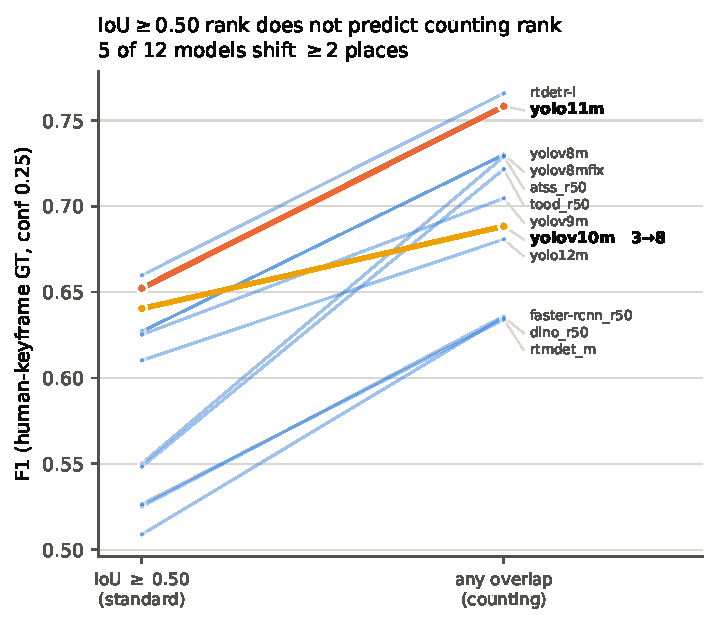
\includegraphics[width=\linewidth]{figures/fig3_criterion.pdf}
  \caption{\textbf{Rank under IoU$\geq$0.50 does not predict rank under the counting
  criterion.} Eight of eleven models shift by two or more places; YOLOv10m falls from 2nd to
  9th. Choosing a detector for a counting system by its detection metric selects the wrong
  model.}
  \label{fig:criterion}
\end{figure}

\Cref{fig:criterion} plots the same data as a rank change. Eight of the eleven models move
at least two places and YOLOv10m falls seven, from 2nd under IoU$\geq$0.50 to 9th under the
counting criterion. Selecting a detector for a counting pipeline on its detection metric
therefore does not select the model that counts best.

We adopt YOLO11m as the production detector for every counting experiment that follows. It
is not the single best model under the counting criterion --- the top five are separated by
0.015 F1, which is inside the noise of a 32-video corpus --- but it has the highest precision
of the roster (0.732), and \cref{sec:counting} shows that precision, not recall, is what the
downstream confirmation stage is starved of.

\subsection{Resolution is architecture-dependent}

\begin{table}[t]
\centering\small
\begin{tabular}{llcccc}
\toprule
Model & res & P & R & mAP50 & AP$_{S}$ \\
\midrule
YOLOv9m & 640 & 0.704 & 0.448 & 0.498 & 0.128 \\
\textbf{YOLOv9m} & \textbf{1280} & \textbf{0.757} & \textbf{0.491} & \textbf{0.523} & 0.119 \\
YOLOv10m & 640 & 0.674 & 0.455 & 0.498 & 0.117 \\
YOLOv10m & 1280 & 0.670 & 0.432 & 0.458 & 0.093 \\
\bottomrule
\end{tabular}
\caption{\textbf{640 versus 1280\,px.} Higher resolution helps YOLOv9m and \emph{hurts}
YOLOv10m; at 640 the two are tied, at 1280 they diverge by 0.065 mAP50. Note AP$_S$ does not
improve for either, so the small-object deficit is not primarily a resolution deficit.}
\label{tab:resolution}
\end{table}

\Cref{tab:resolution} shows that ``higher resolution helps small objects'' does not hold as
a general claim on this data. It helps one architecture and hurts another, and AP-small
declines for both even where overall mAP50 rises. The best detector at 1280\,px (YOLOv9m) is also
not the best counter (\cref{sec:counting}), an early instance of the divergence this paper
characterizes.
